\documentclass[11pt]{article}
\usepackage[utf8]{inputenc}
\usepackage[IL2]{fontenc}
\usepackage[czech]{babel}
\usepackage{wrapfig}
\usepackage[dvipdf]{graphicx}
\usepackage{color}
\usepackage{float}
\usepackage{amsmath}
\usepackage{amssymb}
\usepackage{hyperref}

\usepackage[total={15.5cm,23cm}, top=3cm, left=3cm, includefoot]{geometry}

\setlength\parindent{2em}

\usepackage{etoolbox}

\title{KIV/TI: Převod nedeterministického automatu na deterministický}
\author{Jaroslav Klaus, Vladimír Láznička}
\begin{document}
\begin{titlepage}

\includegraphics[width = 6cm]{logo_fav.jpg}
\begin{center}
\vfill
\textsc{\large KIV/TI - Teoretická informatika}\\
\textsc{\LARGE Převod nedeterministického automatu na deterministický}
\\[0.2cm]
\end{center}
\vfill
Jaroslav Klaus (A13B0347P), Vladimír Láznička (A13B0371P)
\\[0.2cm]
18. ledna 2015,  Plzeň
\end{titlepage}

\tableofcontents

\newpage

\section{Zadání}
Implementujte algoritmus pro převod nedeterministického koneèného rozpoznávacího automatu (umožněte i existenci e-hran) na ekvivalentní deterministický automat. Navrhněte vhodný formát vstupních a výstupních dat.

Program odlaďte alespoň na 6 příkladech včetně příkladů prezentovaných na přednáškách a cvičeních.

Všechny testovací příklady uveďte v dokumentaci včetně ručního řešení.

\subsection{Formát vstupních a výstupních dat}
Jako formát vstupních a výstupních dat budeme volit textové soubory \texttt{*.TI} odpovídající definici nedeterministického konečného rozpoznávacího automatu (vstup) a deterministického konečného rozpoznávacího automatu (výstup) na stránce \url{http://home.zcu.cz/~vais/formaty.htm}. Cílem výstupu je pak možnost jej využít pro další zpracování (např. minimalizace) daného automatu dalším programem.

\newpage

\section{Analýza}
Řešení úlohy lze rozdělit do následujících celků - načtení dat ze vstupu a jejich zpracování do příslušné struktury, samotný převod automatu podle dané reprezentace na deterministický typ, uložení dat vzniklých z převodu do příslušné struktury a nakonec výpis výsledku na výstup.

\subsection{Zpracování vstupu}
Pro zpracování vstupu bude zapotřebí připravit si funkci nebo metodu, která provede parsování vstupu na jednotlivé řetězce, ze kterých se poté získají hodnoty důležité pro reprezentaci automatu a jeho následný převod. Formát vstupního souboru bude naprosto zásadní dodržet, neboť v opačném případě může dojít k chybnému převodu nebo také k němu nemusí dojít vůbec. Vstupní soubor nám udává počet stavů automatu, velikost množiny vstupních symbolů, přechodovou tabulku automatu a nakonec výpis vstupních a výstupních stavů. Tyto informace bude třeba uložit do struktury nebo objektu reprezentující daný automat. Jako reprezentace automatu se pak využije zmíněná přechodová tabulka, která v sobě drží defacto všechny potřebné informace k jeho převodu na deterministický typ. Ostatní informace poslouží buď k vytvoření dalších celků (jako velikost polí na základě počtu stavů) nebo k závěrečné části převodu - určení vstupního stavu a výstupních stavů deterministického automatu. Samotný seznam stavů nebude ke způsobu zápisu vstupního souboru potřeba, neboť stavy vždy odpovídají velkým písmenům a jsou řazené podle abecedy (obdobně to platí pro množinu vstupních symbolů, nicméně tu nebudeme pro převodu automatu přímo potřebovat).

\subsection{Převod nedeterministického automatu na deterministický}
Převod bude probíhat pomocí přechodové tabulky, která se bude postupně upravovat, aby se z ní odstranily všechny nedeterminismy (více vstupních stavů, nejednoznačné přechody a přítomnost e-hran). To nám zajiští jistou inuitivnost a umožní snazší porovnání s ručním řešením, které bude rovněž prováděno na základě přechodové tabulky.

Při vytváření tabulky deterministického automatu se nejprve použije první řádek tabulky z původního automatu, který se bude procházet položku po položce, z nichž se vyberou ty stavy, které ještě nemáme zaznamenány (na počátku máme pouze jeden vstupní stav). Pokud bude položka obsahovat více stavů, tyto stavy se spojí v jeden nový stav a ten se zaznamená. Pro každý takto zaznamenaý stav se vytvoří další řádek, jeho položkky budou obsahovat stavy, do kterých bychom se z něj dostali v daném nedeterministickém automatu pomocí příslušného vstupního znaku. Pokud byl nově vzniklý stav z více původních stavů, v položkách pro tento stav budou zaznamenány stavy, do kterých se lze daným znakem dostat ze všech těchto původních stavů. Takto se bude pokračovat, dokud nebudou nalezeny všechny nové stavy a pro ně vytvořeny příslušné položky.

V případě více vstupních stavů se tyto stavy na počátku přechodu spojí v jeden a takto vzniklý stav se použije jako první zaznamenaný. Pokud bude nedeterministický automat obsahovat e-hrany, což je indikováno další položkou pro příslušný stav v původní přechodové tabulce (jejich počet pak o 1 přesahuje uvedenou velikost množiny vstupních znaků), budeme vytvářet navíc tzv. tabulku e-následníků, která bude pro každý stav z původního automatu uvádět, do jakých dalších stavů se lze dostat prostřednictvím e-hrany (včetně jeho samého). Tyto stavy se pak sjednotí do jednoho nového, který bude mít vlastnosti všech v sobě obsaženách stavů a bude reprezentovat původní stav, pro nějž se tito e-následníci zjišťovali.

Jakmile budeme mít vytvořenou přechodovu tabulku deterministického automatu, určíme pomocí seznamu výstupních stavů z nedeterministického automatu, jaké stavy budou výstupní v deterministickém automatu. Budou to ty, které v sobě obsahují nějaký výstupní stav z původního automatu. Jako stav vstupní se použije buď ten původní, pokud byl jeden, nebo stav vzniklý sjednocením několika původních stavů, pokud jich bylo více.

\subsection{Uložení parametrů deterministického automatu a vypsání výstupu}
Vzhledem k tomu, že z předchozí části již budeme mít všechny potřebné informace - počet stavů, přechodovou tabulku, vstupní stav a výstupní stavy, lze je jednoduše uložit do stejné struktury nebo objektu jako u nedeterministického automatu. Pak už jen stačí použít vhodnou funkci nebo metodu, která si tyto informace vezme a zapíše je do souboru v daném formátu (v zásadě bude fungovat přesně opačně než funkce pro načtení dat ze souboru). 

\newpage

\section{Implementace programu}
K implementaci programu jsme se rozhodli použít jazyk Java, který je jednak výhodný svým objektovým přístupem a také obsahuje několik knihovních tříd umožňující používání různých struktur jako seznamy apod., anož bychom je museli sami implementovat. Nevýhodou je pak samozřejmě pomalejší běh než např. při použití jazyka C, ale pro náš případ není vysoká rychlost zpracování až tak důležitá.

\subsection{Objekt Automaton}
Tento objekt slouží k uchování informací o automatu ve svých atributech. Těmito atributy jsou:

\begin{itemize}
\item \texttt{String automatonType} - řetězec obsahující zkratku typu automatu
\item \texttt{int statusCnt} - počet stavů automatu 
\item \texttt{int inputCnt} - velikost množiny vstupních znaků
\item \texttt{String[][] automatonTable} - pole uchovávající přechodovu tabulku automatu, každý řádek přísluší jednomu stavu (A... Z) a každý sloupec jednomu vstupnímu znaku (a... z).
\item \texttt{ArrayList<String> inputStatuses} - seznam se vstupními stavy automatu
\item \texttt{ArrayList<String> outputStatuses} - seznam s výstupními stavy automatu
\end{itemize}

Dále má samozřejmě metody pro ukládání a vracení těchto atributů, kde je to třeba. Konstruktor pak jako parametry přijímá zkratku automatu, počet stavů a počet vstupních znaků.

\subsection{Načtení souboru a uložení dat}
Načtení souboru je řešeno pomocí metody \texttt{static createAutomatonFromFile(String filePath)}, která přebírá jako parametr řetězec s cestou ke vstupnímu souboru a je obsažena ve třídě \texttt{Input\_Output}. Metoda používá ke čtení souboru knihovní třídu \texttt{BufferedReader}, zejména její metodu \texttt{readLine()}, pomocí které získa řetězec představující obsah aktuálně načítaného řádku. Ten je pak rozdělen buď ručně nebo pomocí metody \texttt{split()}, přičemž jako dělící znak je použita mezera. Nejprve se načte typ automatu, počet stavů a počet vstupních znaků a tyto hodnoty se poté použijí k vytvoření objektu \texttt{Automaton}. Následně se načte přechodová tabulka a postupně uloží do dvourozměrného pole řetězců, které se pak objektu předá. Nakonec se načtou vstupní a výstupní stavy do příslušných seznamů a rovněž se předají objektu.

\subsection{Algoritmus převodu}
- doplnit -

\subsection{Uložení výsledného automatu a výpis na výstup}
Výsledný deterministický automat je vytvořen na konci metody pro převod. Nejprve se vytvoří objekt tohoto automatu, přičemž jako parametry jsou použity řetězec "DKAR" (deterministický konečný automat rozpoznávací - dle požadovaného formátu souboru), velikost seznamu s vytvořenými stavy a počet vstupních znaků z původního automatu (ten se převodem nijak nemění). Poté se uloží pomocí metody \texttt{static void setOuputStatusesToDka(Automaton nka, Automaton dka, LinkedList<String> statuses)} seznam výstupních stavů automatu postupem víceméně popsaným v analýze. V metodě také dojde k přejmenování stavů tak, aby vyhovovaly formátu souboru, který bude výstupem. Přejmenování probíhá procházením vytvořených výstupních stavů, které mohou být v tu chvíli označené jako složení původních stavů, přičemž se tyto stavy porovnávají se seznamem všech nově vytvořených stavů a jakmile dojde ke shodě, složený stav se přejmenuje podle formule \texttt{'A'+ index stavu v seznamu vytvořených stavů}. K podobnému přejmenování dojde i ve vytvořené přechodové tabulce v metodě \texttt{static void renameStatuses(String[][] dkaTable, LinkedList<String> statuses)}. Nakonec se tabulka předá objektu automatu a tytvoří se list s jednim stavem \texttt{"A"}, který je uložen jako vstupní (prezentuje množinu původní vstupních stavů).

Objekt se pak použije k výpisu informací do výstupního souboru pomocí metody \texttt{static void writeAutomatonToFile(Automaton a, String filepath)} ze třídy \texttt{Input\_Output}. V zásadě funguje opačně než metoda pro získání dat ze souboru. Postupně skládá informace získané z objektu automatu do řetězců, představující jednotlivé řádky (podle požadovaného formátu) a ty pomocí metody \texttt{write(<retezec>)} z knihovní třídy \texttt{BufferedWriter} zapisuje do zadaného souboru. 
-doplnit-

\newpage

\section{Uživatelská dokumentace}

-doplnit, podle domluvy-

\newpage

\section{Porovnání s ručním řešením převodu a ověření správnosti}

-doplnit-

\newpage

\section{Závěr}

-doplnit-

\newpage




Řešení zadané úlohy lze rozdělit do několika funkčních celků – rozhodnutí, čím se bude \textbf{síť reprezentovat v~programu}, resp. paměti počítače (soustava polí nebo řada na sebe navazujících spojových seznamů apod.), zjištění \textbf{parametrů výsledné neuronové sítě} (jako kolik bude mít vrstev a kolik neuronů bude obsahovat každá vrstva), \textbf{sestavení její struktury} na základě údajů získaných z~předchozí části s~využitím vhodných struktur, \textbf{uložení dat přečtených ze vstupních souborů do zmíněných struktur} a nakonec \textbf{výpočet aktivačních hodnot na základě přečtených dat} a poskytnutého výpočetního vzorce.

\subsection{Reprezentace sítě v~programu}
Reprezentaci sítě v~programu je třeba navrhnout především s~ohledem na jednoduchost jejího vytvoření a především potom na efektivitu závěrečného výpočtu. Je třeba sestavit jednotlivé vrstvy, jejich neurony a hrany mezi neurony do příslušné konstrukce tak, aby bylo umožněno nenáročné přecházení mezi těmito strukturami při následném ukládání přečtených dat a při výpočtu aktivačních hodnot.

V~zásadě se nabízejí dvě hlavní možnosti – buď reprezentace sítě pomocí \textbf{soustavy spojových seznamů}, kdy do sítě se lze dostat přes seznam s~vrstvami, přičemž z~každé vrstvy povede ukazatel na první člen seznamu s~neurony a od každého neuronu pak povede ukazatel na první člen seznamu s~hranami, vedoucími do daného neuronu. Tato struktura pak nabízí jistou flexibilitu v~tom smyslu, že v~zásadě nemusíme dopředu řešit, jak velká síť bude, před jejím sestavením z~příslušných struktur (mohli bychom tedy v~podstatě vypustit část se zjišťováním parametrů sítě). Na druhou stranu nám zase nenabízí možnost se snadno dostat na nějaký specifický člen některé ze struktur bez toho, aniž bychom potřebovali vždy prohledávat příslušný seznam, což by způsobovalo pomalejší běh zejména v~části provazování neuronů hranami (hrany pravděpodobně budou nejpočetnější množinou v~síti).

Druhá možnost je pak reprezentovat síť pomocí \textbf{soustavy polí}. To nám poskytne výhodu v~možnosti dostat se na nějakou specifickou strukturu pomocí indexu, což zefektivní některé části programu. Na druhou stranu potřebujeme pak vědět dopředu, jak bude neuronová síť velká, abychom mohli přiřadit polím se strukturami přesně velkou paměť. Hrany mezi neurony pak budou stále muset být reprezentovány spojovým seznamen, protože nelze snadno zjistit jejich počet u~každého z~neuronů. Na druhou stranu při jejich přidávání do seznamu nebo následném výpočtu nebude třeba znát nějaký index konkrétní hrany, neboť budeme vždy procházet jednu po druhé.

V~případě využití konstrukce sítě pomocí polí u~vrstev a jejich neuronů lze ještě uvažovat o~\textbf{matici neuronů}, kdy první index bude představovat vrstvu a druhý index jejího neuronu. Výhoda je potom taková, že v~zásadě není zapotřebí definovat strukturu pro samotné hrany a celkové zjednodušení schématu při implementaci, ale dost značná nevýhoda je ta, že velikost matice bude daná vrstvou s~největším počtem neuronů a u~ostatních vrstev nebude paměť zcela využita. Matice je pak speciálně nevýhodná v~případě, kdy jsou mezi počtem neuronů v~jednotlivých vrstvách propastné rozdíly.

Pro další části budeme počítat s~reprezentací pomocí \textbf{polí u~vrstev a neuronů a spojového seznamu u~hran mezi neurony}.

\begin{figure}[htbp]
\centering
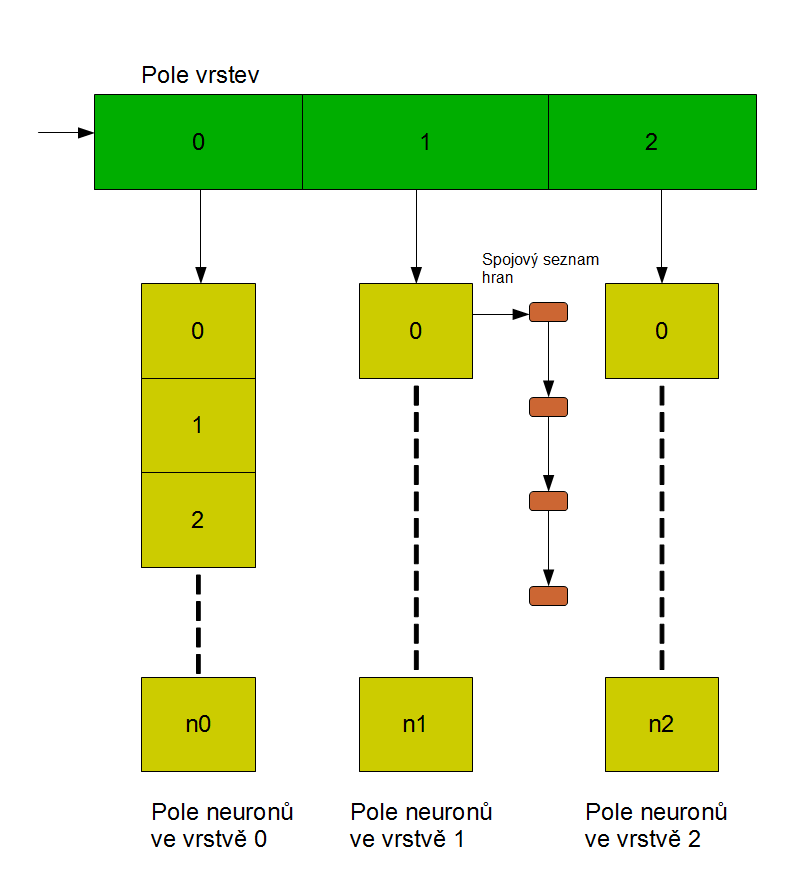
\includegraphics[width = 15cm]{PCschema.png}
\begin{center}
\caption{Schéma neuronové sítě popsané v~analýze}
\end{center}
\end{figure}

\subsection{Parametry připravované sítě}
Pro zjištění parametrů potřebných pro následné sestavení neuronové sítě bude zapotřebí provést \textbf{předběžné čtení souborů}. Ze \textbf{souboru s~aktivačními hodnotami} pro vstupní vrstvu bude zapotřebí zjistit \textbf{počet hodnot}, které soubor obsahuje, tato hodnota nám pak bude indikovat, kolik neuronů se nachází ve vstupní vrstvě. Ze \textbf{souboru s~topologií sítě} poté zjistíme, kolik vrstev bude následovat po vstupní vrstvě a kolik neuronů bude každá z~nich obsahovat. Počet neuronů lze zjistit z~části souboru, kde jsou vypsané \textbf{konstanty} pro každý neuron v~dané vrstvě. Vzhledem k~tomu, že každý neuron má práve jednu takovou konstantu, počet řádek s~nimi v~dané části/vrstvě se pak rovná počtu neuronů.

\subsection{Sestavení neuronové sítě}
Sestavení sítě proběhne v~momentě, kdy budeme znát její parametry (počet vrstev a neuronů) a částečně při čtení hodnot ze \textbf{souboru s~topologií sítě}. Pro vrstvy se vytvoří pole příslušných struktur, kdy každá taková struktura bude obsahovat \textbf{ukazatel na pole} se strukturami reprezentující neurony. Každy neuron pak bude obsahovat \textbf{ukazatel na první člen} spojového seznamu hran, které do něj vedou \footnote{Vzhledem k~uvedenému vzorci výpočtu je výhodnější odkazovat se na seznam hran z~neuronu, pro který chceme vypočítat jeho aktivační hodnotu.}. Do spojového seznamu s~hranami se pak budou přidávat struktury jednotlivých hran podle toho, jak budou postupně čteny ze souboru i s~jejich hodnotami (jaké neurony spojují a jakou mají váhu). Souběžně s~přídáváním hran k~jednotlivým neuronům k~nim budeme přiřazovat v~souboru uvedené konstanty, které se budou při výpočtu sčítat se sumou násobku váhy hrany a aktivační hodnoty neuronu z~předchozí vrstvy, ze kterého hrana vede.

\subsection{Výpočet aktivačních hodnot}
Výpočet aktivačních hodnot pro všechny neurony ve vrstvách následující po vstupní vrstvě by vzhledem ke konstrukci sítě měl být poměrně přímočarý. Postupně budeme procházet jednotlivé vrstvy a pro každý jejich neuron provedeme \textbf{součet násobků váhy jednotlivých hran, k~jejichž spojovému seznamu se lze dostat přes ukazatel uložený ve struktuře neuronu, a aktivačních hodnot neuronu z~předchozí vrstvy, jejichž index v~rámci pole neuronů bude uložen ve struktuře hrany}. K~tomuto součtu se pak přičte na neuronu uložená konstanta a takto se bude cyklicky pokračovat pro všechny další neurony v~dalších vrstvách. Nakonec se určí \textbf{nejvyšší aktivační hodnota u~neuronů poslední vrstvy} a index neuronu s~touto hodnotou se pak vrátí jako výsledek.

\newpage

\section{Implementace programu}
Program se mimo hlavního souboru \texttt{main.c} skládá z~následujících modulů:

\begin{itemize}
\item \texttt{layer.h} a \texttt{layer.c}, které obsahují předpis struktury pro reprezentaci neuronových vrstev a funkcí pro jejich vytváření a pro vytváření polí pro ukazatele na jejich neurony, 
\item \texttt{neuron.h} a \texttt{neuron.c} obsahující předpis pro strukturu reprezentující jednotlivé neurony a funkce pro jejich vytváření,
\item \texttt{edge.h} a \texttt{edge.c} s~předpisem struktury reprezentující hrany mezi neurony a funkcí pro jejich přidávání do spojového seznamu,
\item \texttt{my\_functions.h} a \texttt{my\_functions.c} obsahující funkce pro provedení jednotlivých kroků programu od načtení zdrojových souborů až po výpočet aktivačních hodnot a vrácení výsledku. 
\end{itemize}

Struktura sítě použitá v~programu odpovídá návrhu vybraném v~analýze úlohy – \textbf{pole vrstev a neuronů a spojový seznam hran}.

\subsection{Struktura pro vrstvy sítě}
Struktura reprezentující neuronové vrstvy \texttt{layer} obsahuje jednak \textbf{pole ukazatelů} na její neurony a potom proměnnou typu \texttt{integer} uchovávající informaci o~jejich počtu. Mezi funkce obsažené v~modulu této kontrukce pak patří funkce \texttt{layer *createLayer(int neuron\_count)}, která přijme informaci o~počtu neuronů, alokuje paměť potřebnou pro strukturu \texttt{layer}, uloží informaci o~počtu neuronů do připravené proměnné struktury a vrátí \textbf{ukazatel na danou strukturu}. Další funkcí pak je \texttt{void createNeuronArray(layer *l)} přijímající jako vstupní parametr \textbf{ukazatel na vrstvu}, přičemž alokuje paměť potřebnou pro vytvoření \textbf{pole ukazatelů} na struktury typu \texttt{neuron} a následně volá funkci na vytvoření jednotlivých neuronů a ukládání jejich ukazatelů na jednotlivé indexy v~poli.

\subsection{Struktura pro neurony ve vrstvách}
Struktura reprezentující jednotlivé neurony \texttt{neuron} obsahuje dvě proměnné typu \texttt{double} pro uložení \textbf{aktivační hodnoty a konstanty ze souboru} a \textbf{dva ukazatele na spojový seznam s~hranami} příslušející danému neuronu. Jeden ukazuje na první prvek v~seznamu a druhý na poslední. Ukazatel na poslední prvek seznamu je ukládán pro rychlejší přidávání nových hran do seznamu, není pak zapotřebí procházet všechny již přidané hrany, abychom mohli přidat novou na jeho konec. Funkce, která má za úkol vytvářet neurony \texttt{neuron *createNeuron()} alokuje paměť potřebnou pro tuto strukturu, nastaví oba ukazatele na seznam neuronů na \texttt{NULL} a vrátí \textbf{ukazatel na daný neuron}.

\subsection{Struktura pro hrany mezi neurony jednotlivých vrstev}
Struktura reprezentující hrany \texttt{edge} obsahuje proměnnou typu \texttt{double} pro uložení \textbf{váhy hrany}, proměnnou typu \texttt{integer} pro uložení \textbf{indexu neuronu}, ze kterého hrana vychází \footnote{Ukazatel na seznam s~hranami vždy uchovává neuron, do kterého hrana směřuje, kvůli jednodušší situaci při výpočtu aktivačních hodnot.} a \textbf{ukazatel na následující hranu} v~seznamu. Funkce na přídání nové hrany \texttt{void addEdgeToList(edge **head, edge **tail, double weight, int neuron\_index)} vždy přijme odkaz na \textbf{ukazatel hlavičky a konce seznamu, váhu hrany a index neuronu, ze kterého hrana vychází}. Poté alokuje paměť pro strukturu hrany a vložené hodnoty uloží do proměnných struktury. Následně ověří, jestli již nějaká hrana existuje na ukazateli na hlavičku seznamu, pokud ano, vloží ukazatel na novou hranu do proměnné pro ukazatel na další hranu u~poslední vložené nacházející se na místě, kam ukazuje ukazatel na konec seznamu. V~opačném případě se hlavička i konec seznamu nastaví na právě vkládanou hranu.

\subsection{Postup činnosti programu}
Nyní, když máme popsány jednotlivé struktury nacházející se v~programu, rozebereme si postup funkce programu samotného tak, jak je specifikován ve funkci \texttt{main} (pozn.: všechny další funkce, s~vyjímkou funkcí pro uvolňovaní paměti zabrané výše popsanými strukturami jsou obsaženy v~modulu \texttt{my\_functions}). Program si nejprve zkontroluje, zda byl zadán \textbf{dostatečný počet vstupních argumentů programu}, pokud ne, vypíše chybovou hlášku a svoji činnost ukončí. Následně si pomocí funkce \texttt{fopen} otevře proudy pro čtení ze \textbf{vstupních souborů}, jejichž umístění bylo specifikováno ve vstupních argumentech programu. Pokud jakýkoliv z~nich nebude moci otevřít, oznámí chybu a ukončí svoji činnost.

Následuje volání funkce \texttt{int getInputLayerActivationsCount(FILE *f, int element\_size)}, která má za úkol zjistit, \textbf{kolik aktivačních hodnot} obsahuje soubor s~příponou \texttt{.dat} nebo-li jaký je \textbf{počet neuronů ve vstupní vrstvě}. Tuto hodnotu pak použije k~alokaci paměti pro pole s~hodnotami typu \texttt{float}, kam poté načte aktivační hodnoty z~výše zmíněného souboru, který potom uzavře, neboť již dále není zapotřebí. Poté dojde k~zavolání funkce \texttt{int getLayerCountFromFile(FILE *f, char *space)}, která přečte \textbf{první řádek souboru s~topologií sítě} a zjistí z~něj, kolik vrstev (mimo té vstupní) bude síť obsahovat. Na základě toho pak program alokuje paměť pro \textbf{pole ukazatelů} na struktury \texttt{layer} a u~první z~nich vytvoří pole ukazatelů na struktury \texttt{neuron} na základě hodnoty získané v~předešlé části kódu. Nakonec pomocí funkce \texttt{copyActivationsToLayer(float *activations\_buffer, layer **neural\_layers, int layer\_index)} přenese aktivační hodnoty z~pole, které bylo vytvořeno pro jejich odložení, do \textbf{proměnných těchto struktur}.

Poté se volá funkce \texttt{int createNeuralLayersFromFile(FILE *f, char *space, layer **neural\_layers)}, která má za úkol zjistit, \textbf{kolik neuronů bude každá vrstva obsahovat} a na základě této informace poté vytvořit pole ukazatelů na struktury \texttt{neuron} u~dalších vrstev podobně jako u~té vstupní. Funkce postupně prochází \textbf{soubor s~topologií sítě} řádek po řádku, přičemž ověřuje, jestli se nachází v~části, kde jsou uvedeny hrany mezi neurony dvou vrstev nebo konstanty pro neurony druhé z~nich. Pokud se nachází v~části s~konstantami, \textbf{inkrementuje si proměnnou představující počet neuronů v~aktuálně procházené vrstvě}. Jakmile se opět dostane do části s~hranami, znamená to, že se zjišťují informace o~další vrstvě a tedy je možné použít zmíněnou proměnnou pro alokování paměti pro dané pole ukazatelů na struktury \texttt{neuron}. Funkce takto pokračuje, dokud nepřečte celý soubor a nevytvoří pole pro všechny vrstvy.

Následně je volána funkce \texttt{int createEdgesFromFile(FILE *f, char *space, layer **neural\_layers)}, která přečte daný soubor znovu obdobným způsobem jako v~předchozím případě. Nicméně zde se snaží v~části s~konstantami \textbf{ukládat tyto do již vytvořených neuronů} a v~části s hranami \textbf{přidává nové hrany do spojového seznamu k~jednotlivým neuronům} v~poli. Obě popsané funkce vypisují na konzoli chybovou hlášku v~případě, že narazí při čtení souboru na něco, co nejsou schopny zpracovat, a \textbf{jejich návratová hodnota je pak použita jako indikace ukončení programu}.

Nyní již máme v~podstatě vytvořenou kompletní neuronovou síť, je zapotřebí jen vypočítat hodnoty aktivace u~jednotlivých neuronů v~jednotlivých vrstvách. To má na starost funkce \texttt{void setActivationValues(layer *l\_curr, layer *l\_prev)}, probíhající v~cyklu nad polem ukazatelů na struktury \texttt{layer}. Jejími vstupními parametry je pak ukazatel na vrstvu, \textbf{pro jejíž neurony chceme vypočítat aktivační hodnoty}, a ukazatel na vrstvu předcházející, \textbf{z~jejíchž neuronů potřebujeme tyto hodnoty přečíst a použít pro výpočet}. Funkce provádí výpočet postupně nad všemi neurony dané vrstvy tak, že na neuronu, kde chceme aktivaci vypočítat, prochází seznam hran a jejich váhy násobí aktivací specifického neuronu z~předchozí vrstvy (k~tomu je použit index neuronu uložený ve struktuře hrany). Tyto násobky jsou sčítany do výsledného součtu, ke kterému je poté přičtena konstanta daného neuronu a matematickou funkcí \textbf{tanh} je vypočítána výsledná aktivace.

Poslední část programu před uvolněním zabrané paměti a jeho ukončením je volání funkce \texttt{int getNeuronIndexWithMaxActivation(layer *l)}, která projde poslední vrstvu, porovná aktivační hodnoty jejích neuronů a vrátí \textbf{index toho neuronu, který měl hodnotu nejvyšší}. Index se poté vypíše na konzoli jako výsledek.

Nakonec se postupně uvolní paměť alokovaná jednotlivými strukturami. K~tomu slouží specifické funkce obsažené v~modulech těchto struktur. \textbf{Uvolňování paměti probíhá jakousi kaskádou}, kdy funkce zabývající se „vyšší“ strukturou (vrstva) volá funkci zabývající se „nižší“ strukturou (neuron nebo hrana v~případě, že je vyšší struktura neuron) předtím, než pro tuto svou strukturu uvolní paměť.

\subsection{Využití knihovních funkcí jazyka C}
Na závěr popisu implementace ještě zmínka o~použitých knihovních modulech. Pro práci se soubory jsou využité funkce z~\texttt{stdio.h}, při načítání jednotlivých řádků souboru s~topologií sítě jsou pak pro získávání hodnot použity funkce z~\texttt{string.h}. Dále pro výpočet aktivační hodnoty přes matematickou funkci tanh je zahrnuta \texttt{math.h} a pro definování konstanty \texttt{DBL\_MAX} (použitá při porovnávání aktivací) je zahrnuta \texttt{float.h}.

\newpage

\section{Uživatelská dokumentace}
Sestavení programu ze zdrojových a hlavičkových souborů lze provést pomcí přiložených souborů \texttt{Makefile} (jeden pro systémy \textbf{Windows}, druhý pro \textbf{GNU/Linux}). V~adresáři, kde se soubory nacházejí, je zapotřebí provést příkaz \texttt{make} pro příslušný \texttt{Makefile}, který pak zkompiluje funkční program spustitelný přes soubor \texttt{neural\_net.exe}. Spuštení samotného programu lze pak realizovat opět z~příkazové řádky kdy zadáme název spustitelného souboru a mezerami oddělené dva parametry, přičemž jejich počet a pořadí je naprosto zásadní. Jako první parametr se poskytne cesta k~\textbf{souboru s~topologií sítě}, který je poskytnutý ve formátu \texttt{.txt}. Jako druhý parametr je třeba zadat cestu \textbf{k~souboru, který obsahuje aktivační hodnoty pro neurony vstupní vrstvy} v~hexadecimální podobě a je poskytnutý s~příponou \texttt{.dat}.

\bigskip

Podoba příkazu na spuštení programu je následující: 

\texttt{neural\_net.exe <soubor\_topologie\_site> <soubor\_vstupnich\_aktivaci>}, 

tedy např. \texttt{neural\_net.exe neuronova\_sit.txt vstupy\textbackslash0.dat}.

\bigskip

Pokud uživatel nezadá dostatečný počet perametrů nebo nastane nějaká neočekávaná situace při čtení souborů, \textbf{program skončí výpisem chybové hlášky}. Po správném průběhu programu je na konzoli vypsán index neuronu z~výstupní vrstvy s~nejvyšší hodnotou aktivace, což představuje výslednou třídu zkoumaného obrázku. \footnote{Na základě poskytnutých testovacích dat se jedná o~číslici na obrázku odpovídajícím zadanému vstupu s~aktivačními hodnotami neuronů vstupní vrstvy.}

\bigskip

\begin{figure}[htbp]
\centering
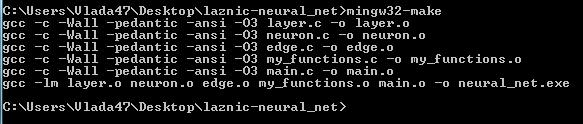
\includegraphics[width = 15cm]{PCmake.jpg}
\begin{center}
\caption{Příkaz pro kompilaci programu a jeho výsledek}
\end{center}
\end{figure}

\begin{figure}[htbp]
\centering
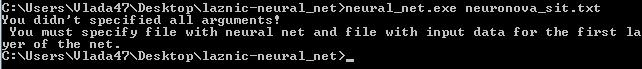
\includegraphics[width = 15cm]{PCerror.jpg}
\begin{center}
\caption{Chybová hláška po zadání nedostatečného počtu argumentů}
\end{center}
\end{figure}

\newpage

\section{Závěr a zhodnocení práce}

Implementace programu splnila předepsané zadání semestrální práce – \textbf{program koretně vytvoří neuronovou síť na základě vstupních souborů a vrátí správný výsledek na konzoli}. Jsou zde samozřejmě místa, která by snesla nějaké to vylepšení, např. minimalizovat počet přístupů do souboru (textový soubor je přečtený dvakrát), což by zkrátilo dobu běhu programu zejména u~velmi velkých sítí s~velkým množstvím hran. Také řešení některých nepředpokládaných situací (zejména chyby ve vstupních souborech nebo problémy s~alokací paměti) by se dalo provést robustněji, ale při korektním použití programu by s~tímto neměl být problém.

Co se týče rychlosti průběhu programu, během testování se jevila jako uspokojivá. Na počítači, kde byl program vyvíjen – dvoujádrový procesor \textbf {Core 2 Duo na taktu 3,5GHz}, \textbf{4GB DDR2} paměti, běžný magnetický disk s~\textbf{7200 ot./min} a operační systém \textbf{Windows} -  byla typická doba provedení všech operací pro poskytnutá testovací data v~průměru kolem \textbf{1,2 sekundy}.

Program by šel samozřejmě dále upravit a optimalizovat pro nižší spotřebu paměti nebo pro větší univerzálnost, ale i tak dokáže dobře řešit zadanou úlohu.

\end{document}